\documentclass[11pt]{article}
\usepackage{graphicx}
\usepackage{listings}
\usepackage{amsmath}
\usepackage{booktabs}
\usepackage{lipsum}
\usepackage[left=1.5cm, right=1.5cm, top=2.5cm, bottom=2.5cm]{geometry}
\title{Hand-in 3}
\author{Michael Iversen\\
Student ID: 201505099}

% Default fixed font does not support bold face
\DeclareFixedFont{\ttb}{T1}{txtt}{bx}{n}{10} % for bold
\DeclareFixedFont{\ttm}{T1}{txtt}{m}{n}{10}  % for normal

% Custom colors
\usepackage{color}
\definecolor{deepblue}{rgb}{0,0,0.5}
\definecolor{deepred}{rgb}{0.6,0,0}
\definecolor{deepgreen}{rgb}{0,0.5,0}

\usepackage{listings}
\usepackage{lipsum}
% Python style for highlighting
\newcommand\pythonstyle{\lstset{
		language=Python,
		basicstyle=\ttm,
		morekeywords={self},              % Add keywords here
		keywordstyle=\ttb\color{deepblue},
		emph={MyClass,__init__},          % Custom highlighting
		emphstyle=\ttb\color{deepred},    % Custom highlighting style
		stringstyle=\color{deepgreen},
		showstringspaces=false
}}

% Python environment
\lstnewenvironment{python}[1][]
{
	\pythonstyle
	\lstset{#1}
}
{}

\begin{document}
\maketitle
In this hand-in, I implement a hidden Markov model following the Codon model from the lectures.
The model contains 5 hidden states: Non-coding, start codon, coding, stop codon, reverse start codon, reverse coding and reverse stop codon.
The non-coding state emits from the alphabet $\mathcal A = \{A, G, C, T\}$ while all other hidden states emits from the alphabet $\mathcal A \times \mathcal A \times \mathcal A = \{AAA, AAG, AAC, AAT, AGA, ..., TTT\}$.
The final model is illustrated in Fig.\ \ref{fig:model} along with the non-zero transition and emission probabilities.
The transition and emission probabilities which are zero have been omitted in this figure.
I obtain the model from training-by-counting without hard-coding any transition or emission probabilities.
A priori, every transition between hidden states and emission of any symbols are allowed.
However, after training, some transitions and emission have probability zero because they didn't appear during training.
\begin{figure}
	\centering
	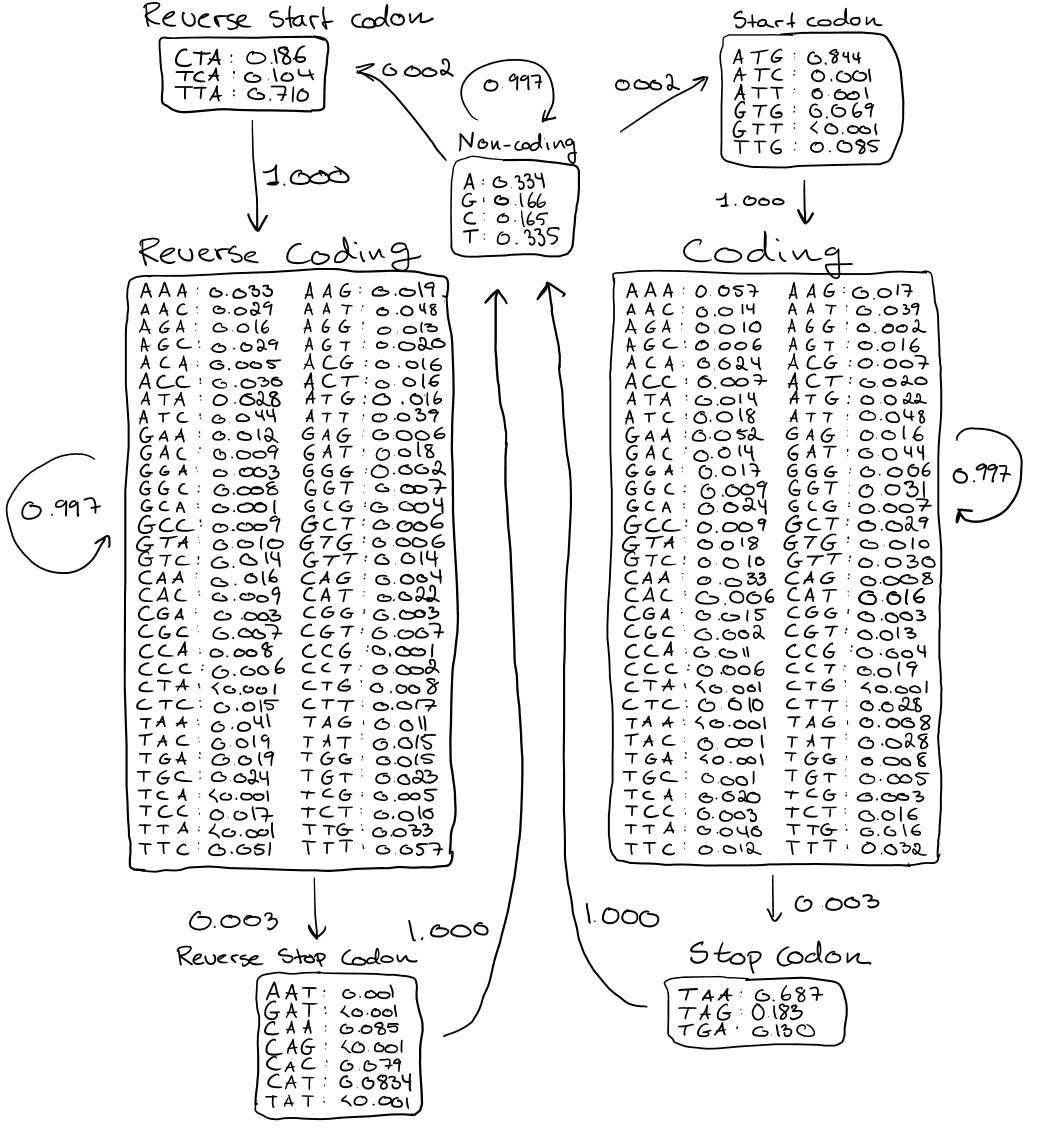
\includegraphics[width=\textwidth]{Illustration.png}
	\caption{
		Model of hidden Markov model with transition and emission probabilities.
		Only non-zero probabilities are shown.
	}
	\label{fig:model}
\end{figure}

I translate the given annotations of non-coding $N$, coding $C$ and reverse coding $R$ into a list of hidden states.
I represent the non-coding state as ``$0$'', start codon as ``$1$'', coding state as ``$2$'', stop codon as ``$3$'', reverse start codon as ``$4$'', reverse coding state as ``$5$'' and reverse stop codon as ``$6$''.
The non-coding part of the annotations are directly translated $N \to 0$.
The start codons are identified as a shift from $N$ to $C$.
Similarly, the stop codons are identified as a shift from $C$ to $N$.
The coding state is determined as part of the annotations where three letters are $C$ with both the preceding 3 and following 3 letters are all $C$.
The reverse start codons, reverse stop codons and reverse coding states are identified using similar considerations.
The code snippet below illustrates this translation.
\begin{python}
def str_to_list(z: str) -> list[int, ...]:
    z_list = []
    n = 0
    while n < len(z):
        if z[n] == 'N':
            z_list.append(0)
            n += 1
        elif z[n] == 'C':
            if 'N' in z[n - 3: n]:
                z_list.append(1)
            elif 'N' in z[n + 1: n + 4]:
                z_list.append(3)
            else:
                z_list.append(2)
            n += 3
        elif z[n] == 'R':
            if 'N' in z[n - 3: n]:
                z_list.append(4)
            elif 'N' in z[n + 1: n + 4]:
                z_list.append(6)
            else:
                z_list.append(5)
            n += 3
    return z_list
\end{python}

Translating a list of hidden states to an annotation in terms of $N$, $C$ and $R$ is straightforward.
I simply map $0 \to N$, $1 \to CCC$, $2 \to CCC$, $3 \to CCC$, $4 \to RRR$, $5 \to RRR$ and $6 \to RRR$.
This procedure is illustrated in the code snippet below.
\begin{python}
def list_to_str(z: list[int, ...]) -> str:
    def decoding(i: int) -> str:
        if i == 0:
            return 'N'
        elif i == 1 or i == 2 or i == 3:
            return 'CCC'
        else:
            return 'RRR'
    return ''.join(map(decoding, z))
\end{python}
\begin{table}
	\centering
	\begin{tabular}{|l|lll|}
		\hline
		\textit{Known genomes} & \textbf{Only Cs} & \textbf{Only Rs} & \textbf{Both} \\ \hline
		\textbf{Genome 1} & $0.7144$ & $0.7675$ & $0.6246$ \\
		\textbf{Genome 2} & $0.7549$ & $0.7411$ & $0.6303$ \\
		\textbf{Genome 3} & $0.7870$ & $0.7751$ & $0.6760$ \\
		\textbf{Genome 4} & $0.7642$ & $0.7379$ & $0.6248$ \\
		\textbf{Genome 5} & $0.7930$ & $0.7390$ & $0.6478$ \\
		\hline
	\end{tabular} \hfill
	\begin{tabular}{|l|lll|}
		\hline
		\textit{Unknown genomes} & \textbf{Only Cs} & \textbf{Only Rs} & \textbf{Both} \\ \hline
		\textbf{Genome 6} & $0.7439$ & $0.7513$ & $0.6356$ \\
		\textbf{Genome 7} & $0.7630$ & $0.7384$ & $0.6380$ \\
		\textbf{Genome 8} & $0.7497$ & $0.7049$ & $0.5993$ \\
		\textbf{Genome 9} & $0.7209$ & $0.6767$ & $0.5297$ \\
		\textbf{Genome 10} & $0.6525$ & $0.6656$ & $0.4576$ \\
		\hline
	\end{tabular}
	\caption{Performance of hidden Markov model on known genomes (left) and unknown genomes (right)}
\end{table}

\end{document}